
A fájlszerkezetnek a tervezésénél nem voltak a belső részek komolyabban megtervezve, dinamikusan változtak. 3 mappa volt a tervezett: elosztott rendszer, weboldal és a külső fájlok mappája. A többi mappa mind a külsők, és a belsők a fejlesztés során lettek bele tervezve, amikor a fájlok mennyisége, vagy az új technológia szeparálása megkívánta azt.

\begin{figure}[h]
	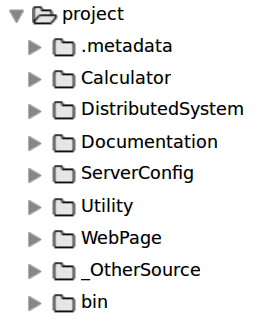
\includegraphics[width=5cm]{pics/folders_all}
	\centering
	\caption{Külső mappaszerkezet\label{fig:folders_all}}
\end{figure}

\begin{description}
	\item[Calculator] \hfill \\ 
		Az interpoláció számítás megvalósítását valamint az Erlang-modullá alakítását is tartalmazó mappa.
		Függvényei a DistributedSystem mappából hívódnak.
	\item[DistributedSystem] \hfill \\ 
		Elosztás logikáját tartamazó mappa, melynek függvényei a ServerConfig mappából hívódnak. 
	\item[ServerConfig] \hfill \\ 
		Szerver megvalósítását tartalmazó mappa.
	\item[Utility] \hfill \\ 
		Több helyen is meghívható függvényeket tartalmazó mappa.
		Struktúra kezelés megvalósítása és a mochijson található itt. 
	\item[WebPage] \hfill \\ 
		Weboldal mappája. 
	\item[\_OtherSource] \hfill \\ 
		Külső felhasznált komponensek mappája.
	\item[bin] \hfill \\ 
		Szerver inicializálását tartalmazó mappa. Ide kerülnek a lefordított fájlok is.
	\item[Documentation] \hfill \\
		Dokumentáció forrás fájljait tartalmazó mappa. 
\end{description}